In this paper we have used two different datasets, for two different purposes. The first dataset is a large dataset containing only the primary structures of proteins, which we will use to train our models. This dataset does not have any information regarding the proteins apart from their primary structure. The second dataset is significantly smaller, consisting also of the primary structures of proteins, but labelled with a value representing the stability of the protein.

\subsection{Training data}
As previously mentioned, we mainly focused on the training of our models with unsupervised learning. There is a lot more data explaining the primary structure of the protein, since this is historically very easy to find, compared to finding secondary structure. \\

\noindent
Since we wanted to replicate the work of UniRep, we also chose to use UniRef50 as our training dataset.\cite{uniref} This dataset contains the primary structures of roughly \~ 27 million proteins. Due to hardware contstraints, we have decided to randomly sample 100,000 sequences from the same dataset, and use this as our training data. \\
Since we do not know how the data has been generated, we chose to randomly sample from the data, instead of taking 100k adjacent samples. We did this to avoid any kind of bias the data could have. For example, the first 100k rows of the dataset could potentially only contain one kind, or simpler and easier to process proteins. This could have an effect on the networks performance, which we have hopefully.\\

\noindent
UniRep removed proteins containing amino acid symbols (X, B, Z, J), and sequences longer than 2,000 amino acids.\cite{unirep} In our case, due to limited hardware and computer power, we chose to remove all sequences longer than 500 amino acids, and sequences containing the (X, B, Z, J) amino acids as well. The sequences containing (X, B, Z, J) are removed because they are considered "non-canonical", meaning that some of them are placeholders etc.\\

\noindent
With the sample reduction, we ended up having roughly 78,000 protein sequences in our training set. We realise that only looking at sequences with a maximum length of $500$ means that we have potentially introduced some bias into the network. This bias may make itself visible when predicting on longer proteins, where the model may think that the sequence has to end at around 500 amino acids. We argue that, in our case at least, this tradeoff is worth it because training is significantly faster, especially for the LSTM.\\

\noindent
The primary structure consists of amino acids. Each amino acid is represented as a char \\ $\in \{A, C, D, E, F, G, H, I, K, L, M, N, O, P, Q, R, S, T, U, V, W, Y\}$. Meaning that each protein from the dataset is represented as a sequence of chars, with arbitrary length. Since the length of each sequence varies, we've added a padding element (padding element is '-'); padding this element on all sequences, resulting in all sequences has a 500 feature-length. Figure ~\ref{fig:before}, shows the frequency of each amino acid in the whole dataset.\\

\begin{figure}[!ht]
  \centering
  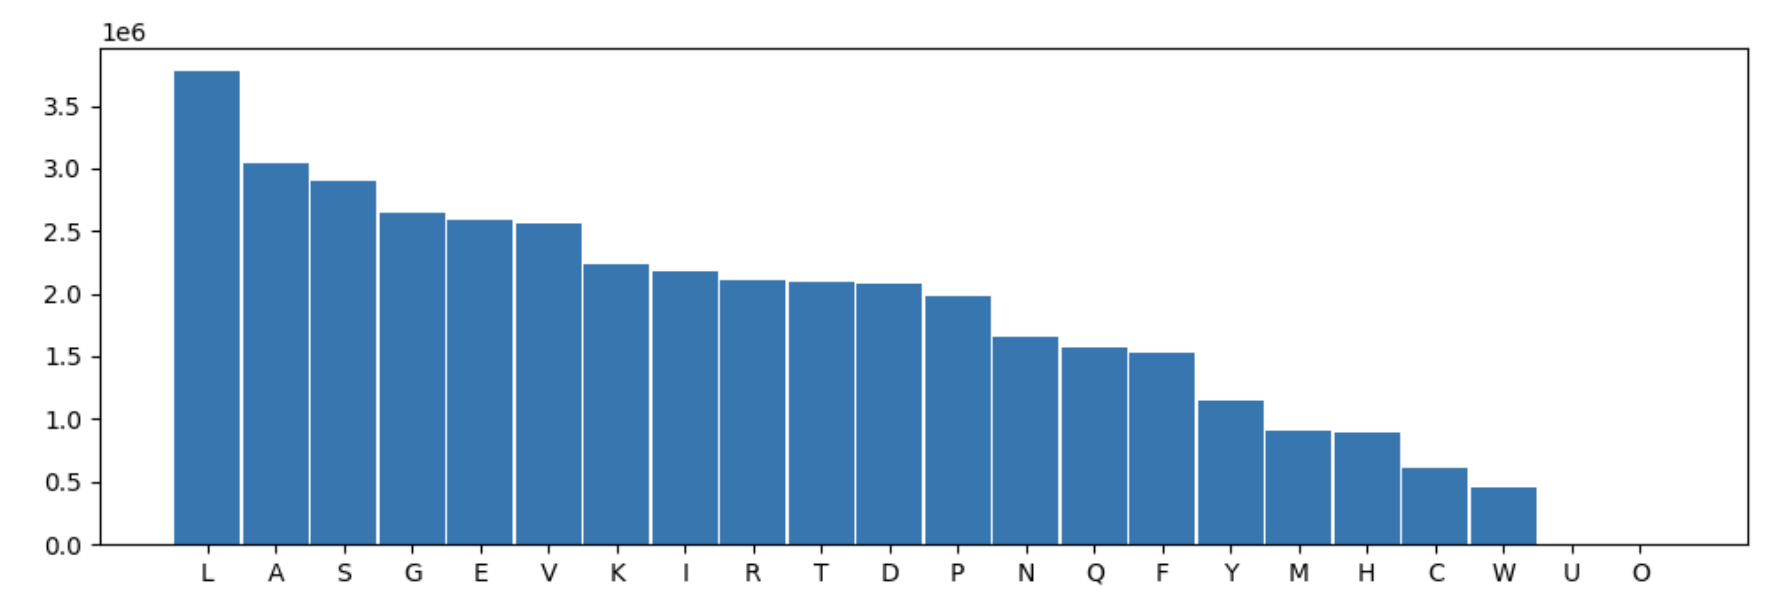
\includegraphics[scale=0.4]{latex/imgs/aminoFreq.png}
  \caption{Histogram of amino acid frequency}\label{fig:before}
\end{figure}

\noindent
Our models use embeddings, which is a method of converting a list of one-hot indices, to corresponding word embeddings. In our case, this meant that we had to transform our sequences into one-hot indices. A one-hot encoding is a way to represent the data, through a vector representation only containing \{0,1\}. Say each protein sequence only contain three amino acids (A, C, D), these amino acids will have the following one-hot encodings.

$$
A = \begin{bmatrix}
1 \\
0 \\
0
\end{bmatrix},
C = \begin{bmatrix}
0 \\
1 \\
0
\end{bmatrix},
D= \begin{bmatrix}
0 \\
0 \\
1
\end{bmatrix}
$$

\noindent
If we were looking at four amino acids (A, C, D, E), the one-hot encoding would look like:

$$
A = \begin{bmatrix}
1 \\
0 \\
0 \\
0
\end{bmatrix},
C = \begin{bmatrix}
0 \\
1 \\
0 \\
0
\end{bmatrix},
D= \begin{bmatrix}
0 \\
0 \\
1 \\
0
\end{bmatrix},
E= \begin{bmatrix}
0 \\
0 \\
0 \\
1
\end{bmatrix}
$$

\noindent
We are having working with 22 amino acids and a pad-value each amino acid will be represented $1$x$23$ onehot encoding. The onehot index describes at which index the $1$ is placed. thus if we define the onehot index of any input as $h$, we get:

\begin{align}
h(A) = 0 \\
h(C) = 1 \\
h(D) = 2 \\
h(E) = 3
\end{align}

\noindent
This means our data gets transformed to one-hot indices before we can use it in our models.

\subsection{Labelled test sets}
Since our models performance is not measured directly on the same kind of data that we trained on, we have two datasets to use as test sets. These datasets labelled, in contrast to the training set. The first dataset has labelling detailing the structural classification of each protein.\cite{scope} The second dataset has labels describing the stability of the given proteins.\cite{stability} Both of these datasets contain the proteins' primary structure in the same format as the training dataset.\\

\noindent
\subsubsection{Structural classification}
We do not use this dataset for quantitative performance analysis however. We instead put the models' representation of the dataset through a TSNE dimensionality reduction to see whether the different structural classifications are clearly separated. 
%Once the model had trained with the training data. We used some labeled data to test the effectiveness of our models. this data also contains protein sequences with the same format as the training data. This data also contains a label, explaining which structure the protein has. This data made it possible to check if our models can find any separation between the different structures.

\subsubsection{Stability}
This dataset is used to quantify the performance of our models. In this dataset, the label explains the stability of the protein. This label is explained with some real number value, which explains how stable some protein is.
%The stability dataset is also labeled dataset containing previously explained protein sequences.  This dataset we use, to check whether or not our models have learned enough of the underlying structure of the proteins, to be used to check the stability of the protein